\section{The Compact Muon Solenoid}
\label{sec:CMS}

CMS is a general purpose detector, designed to be able to perform precision measurements of the standard model and searches for new physics. 
It is a cylindrical, hermetic detector composed of a barrel region and two endcaps, each formed of layers of subdetectors around the beam collision point, as shown in Fig. \ref{fig:CMSPicture}. 
These subdetectors, in order from the collision point, are the pixel and strip tracker, electromagnetic calorimeter (ECAL), hadronic calorimeter (HCAL) and muon chambers.

CMS uses a right-handed coordinate system, where the $x$-axis points towards the centre of the accelarator ring, the $y$-axis points vertically upward and the positive $z$-axis lies parallel to the anti-clockwise beam axis. 
The azimuthal angle, $\phi$, is measured from the $x$-axis in the tranverse $x-y$ plane. 
The polar angle, $\theta$, is measured from the positive $z$-axis in the $z-y$ plane.
At the CMS experiment, collisions are viewed in the centre-of-mass frame of the colliding protons, which means that the colliding partons usually have a boost along the beam direction.
For this reason, the angles of the particles are normally expressed in terms of the rapidity ($y$) or pseudorapidity ($\eta$), in which the production is roughly constant.  
The rapidity is defined as:
\begin{equation}
\label{eq:rap}
y\equiv {\frac{1}{2}}\ln\left({\frac{E+p_{z}}{E-p_{z}}}\right),
\end{equation}
where $E$ is the energy of a measured particle and $p_{z}$ is the $z$-component of the momentum.
Rapidity is advantageous to use as the rapidity difference between two particles is invariant under a lorentz boost along the $z$-axis.
At the LHC, most particles are highly relativistic so that the rest mass is small compared to the energy such that $p_{z}\approx E\cos(\theta)$. This can be substituted into Eq.\,\ref{eq:rap} and using trigonometric relations, the pseudorapidity can be defined as:
\begin{equation}
\label{eq:eta}
\eta \equiv -\ln\left(\tan\left({\frac{\theta}{2}}\right)\right)
\end{equation}

% Henceforth, angular measurements are given in terms of pseudorapidity.
Jet production in \pp{} collisions is roughly constant in $\eta$, reflecting the forward nature of the production.
The subsystems at the CMS experiment extend to at least a pseudorapidity of 2.4, covering more than 95\% of the full phase space. 
Individual subsystems can extend to a higher $\eta$, for example the forward detectors of the HCAL, to study very boosted jets or the underlying event.
Acceptence within $\eta < 2.4$ can be hampered by issues such as the gap between barrel and endcap detectors.
% 2.4 => 10deg. 1 str=33 deg. lost=0.61str. pc = 4.8

To describe the full kinematical properties of a particle, its energy and momentum must be known. 
While it is not possible to detect the complete momenta spectrum of an event, due to many particles produced in the collision being lost down the beam pipe, it is possible to measure the momenta in the transverse plane, where the sum of the momenta is conserved. 
To measure the momentum and energy of a particle, CMS uses a combination of tracks left by charged particles and energy deposits in calorimeters.
These subsytems are described in more detail in the following sections.

\begin{landscape}
\centering
\begin{figure*}[htpb]
	\centering
	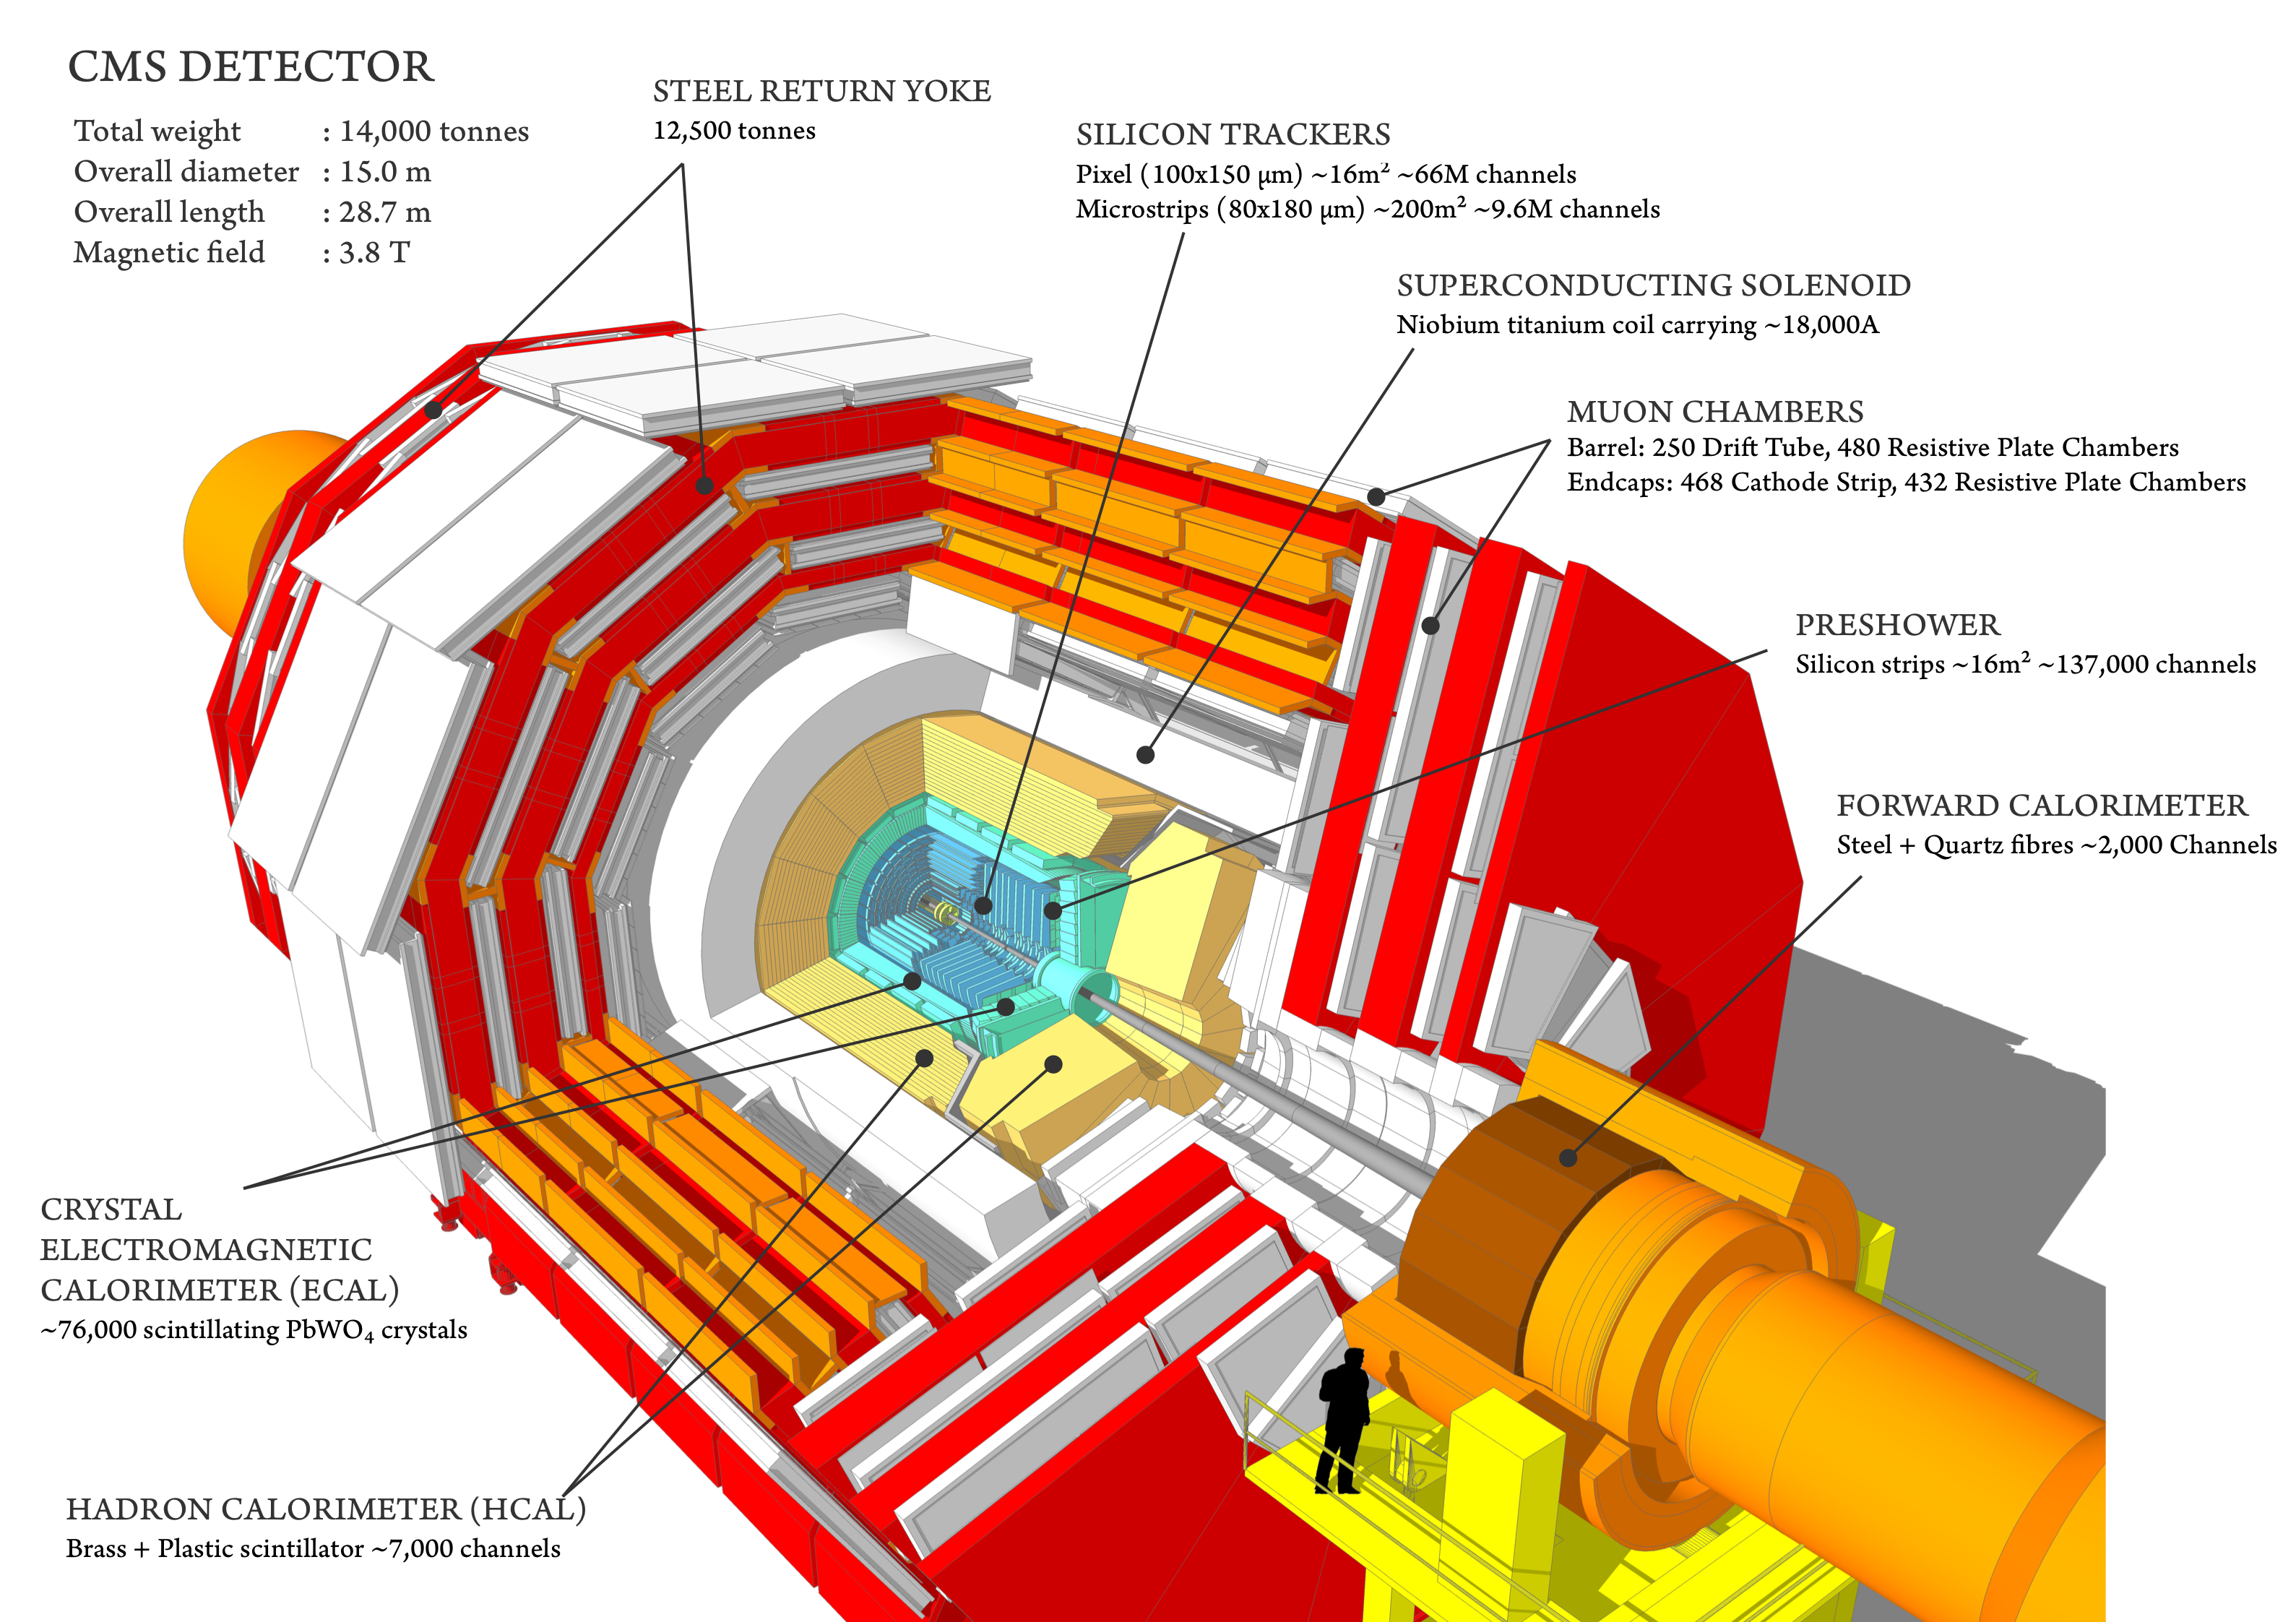
\includegraphics[width=0.8\linewidth]{Figures/CMSPicture}
	\caption[A schematic of CMS, sliced to show the internal layout]{A schematic of CMS, sliced to show the internal layout \cite{CMSPicture}.}
	\label{fig:CMSPicture}
\end{figure*}
\end{landscape}

\subsection{CMS pixel and strip trackers}
\label{ssec:Tracker}
% Page 62

Figure\,\ref{fig:CMSTracker} shows the layout of the silicon tracking detectors in CMS. 
Closest to the interaction point are the pixel detectors consisting of three barrel layers situated at $r=4.4\cm, 7.3\cm$ and 10.2\cm{} in the tranverse plane from the interaction point with two endcap disks lying at $z=\pm34.5\cm$ and $\pm46.5\cm$.  
Surrounding the pixel detectors are the silicon strip tracker sensors. 
These are arranged into four subsystems: the Tracker Inner Barrel and Disks (TIB and TID), the Tracker Outer Barrel (TOB) and the Tracker Endcaps (TEC).
The TIB consists of four barrel layers between $20<r<55\cm$ with each end capped by 3 disks ($|z|<118\cm$) forming the TID. 
Wrapping around the TIB and TID, is the TOB consisting of six barrel layers between $55<r<116\cm$. 
Finally, the TEC extends in nine disks between $124<|z|<282\cm$.
Some strip layers in the tracker, coloured blue in Fig. \ref{fig:CMSTracker}, have back-to-back modules, rotated with respect to each other by a small stereo angle ($\approx5\de$) in order to calculate a hit in 3-dimensions.

\begin{figure}[htpb]
	\centering
	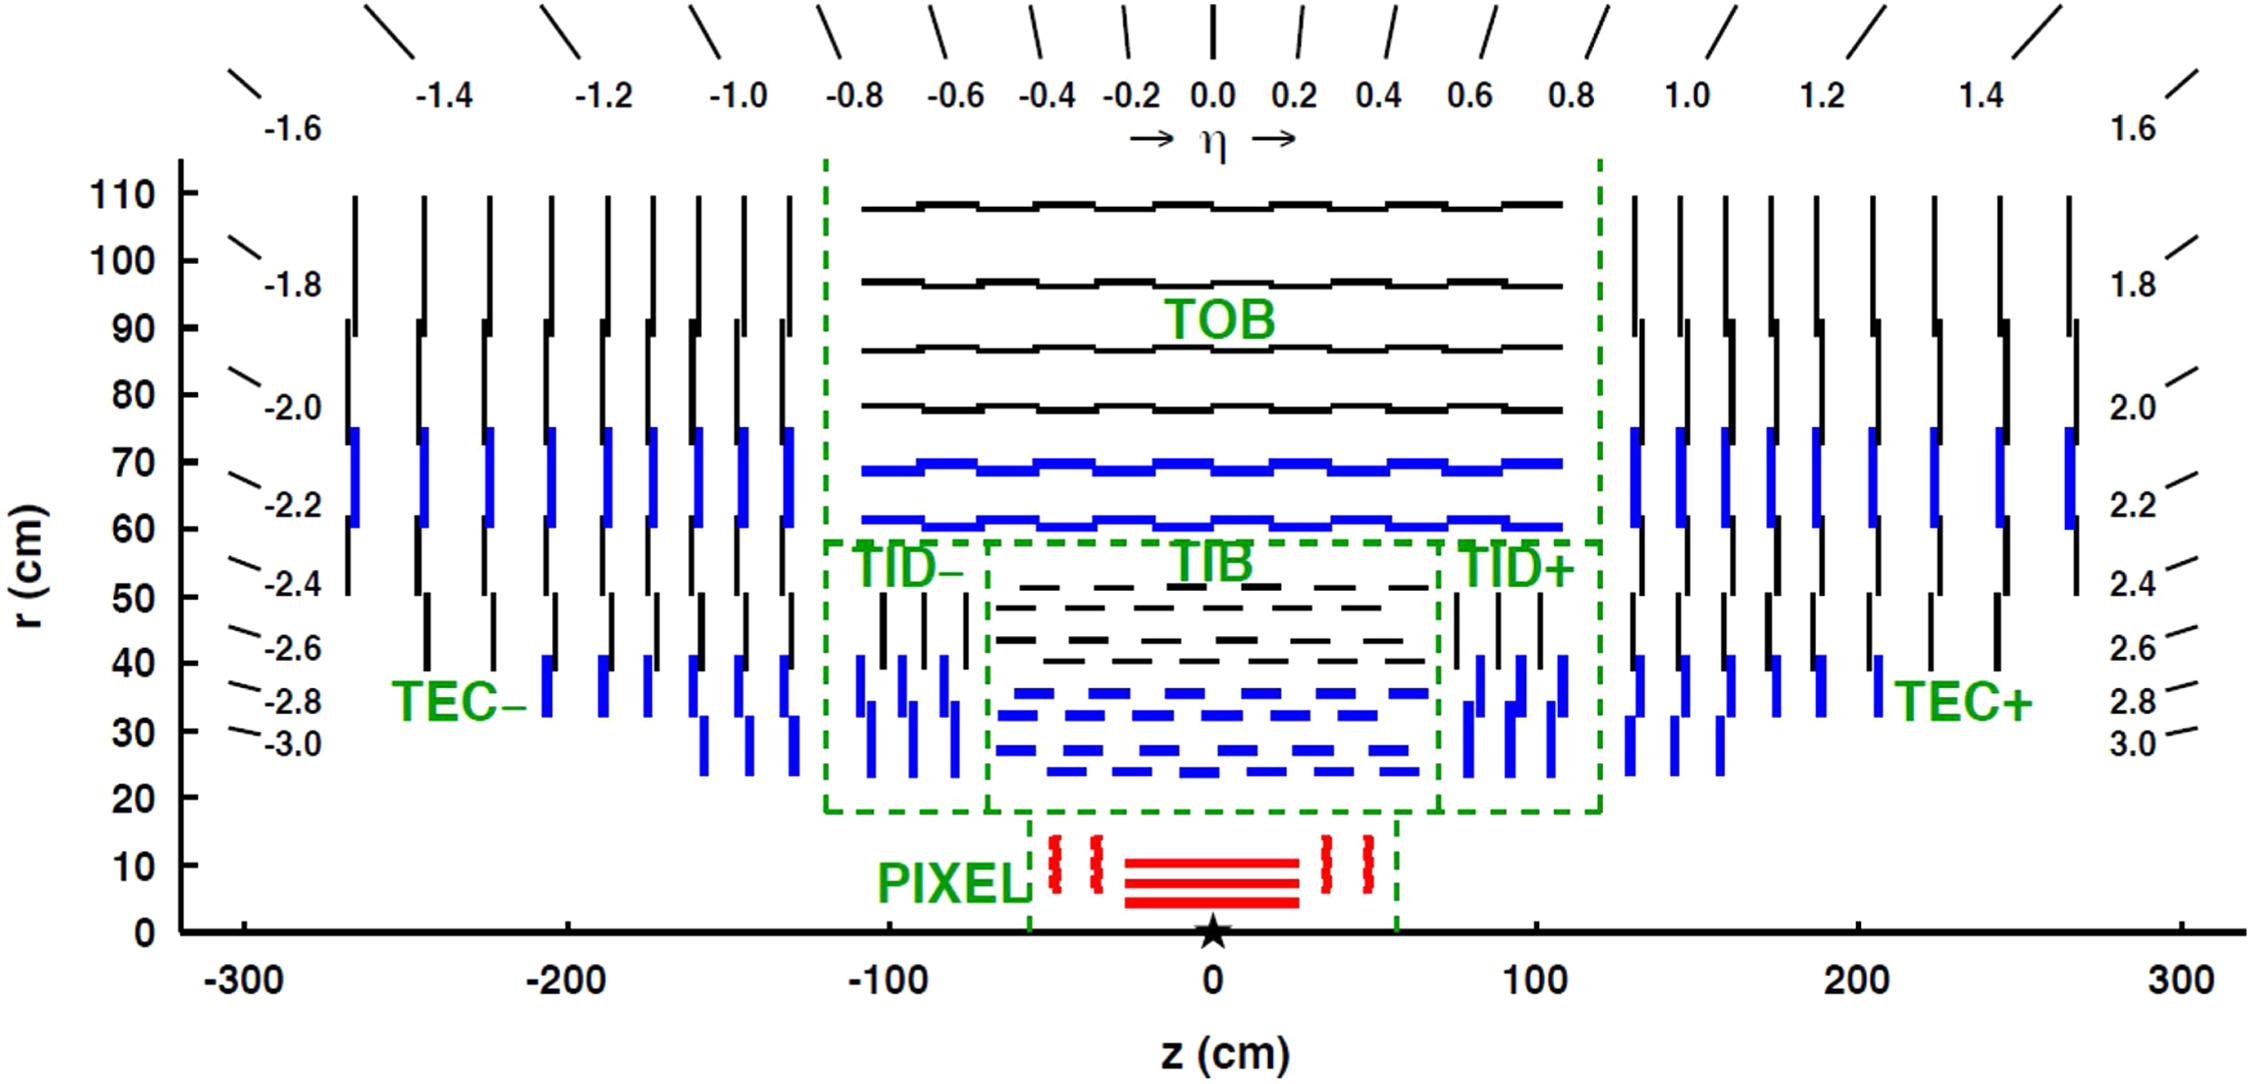
\includegraphics[width=\textwidth]{Figures/CMSTracker2.jpg}
	\caption[The layout of the upper half of the CMS tracker detector in the $r-z$ plane. The separate subsystem regions have been highlighted and are classified as the Tracker Inner Barrel and Disks (TIB and TID), the Tracker Outer Barrel (TOB) and the Tracker Endcaps (TEC). The Pixel subsystem is highlighted in red. Back-to-back stereo strip modules are highlighted in blue.]{The layout of the upper half of the CMS tracker detector in the $r-z$ plane. The separate subsystem regions have been highlighted and are classified as the Tracker Inner Barrel and Disks (TIB and TID), the Tracker Outer Barrel (TOB) and the Tracker Endcaps (TEC). The Pixel subsystem is highlighted in red. Back-to-back stereo strip modules are highlighted in blue. Figure taken from\,\cite{CMSTrackerPerformance}.}
	\label{fig:CMSTracker}
\end{figure}
% of size $100\times150$ $\mu m^{2}$, uses 

Each tracking sensor operates in a similar manner.
For the pixel sensors, an \nnjunc{} junction is utilised where the silicon has been doped with phosphorous to different degrees. 
For the strip sensors, a \pnjunc{} junction is used where a silicon strip doped with boron has been laid on the bulk n-type silicon.
Doping with phosphorous causes the silicon to become an electron donor (n-type) and doping with boron to become an electron acceptor (p-type).
n(p)$^{+}$-type silicon is where silicon has been doped to such an extent that the resisitivity is very low, resulting in a very good chip readout connection.

In the case of the silicon strip sensor, electrons diffuse from the bulk n-type silicon to the strip p$^{+}$-type silicon, creating a small opposing electric field from the formation of ions either side of the \pnjunc{} junction.
The field stops further electron-hole movement and forms a potential step.
The region with no excess electrons or holes is known as the depletion zone, which causes the junction to act as a diode.
A reverse bias voltage is applied to ensure the silicon is fully depleted by attracting the free electrons and holes away from the \pnjunc{} junction.
% A reverse bias voltage is applied to counteract this electric field, increasing the size of the stable depletion zone.
% The reverse bias voltage causes the p$^{+}$-type silicon strip to act as a diode, cutting any... TODO.
When a charged particle ionises the n-type bulk silicon, the electrons and holes produced ($\approx 30,000$) drift in the large electric field such that the holes move towards the p$^{+}$-type silicon producing a small signal current which is then amplified and shaped.
This method can be applied to any semiconductor junction where each side has different doping concentrations.

The pixel detector receives a charged particle flux of $1\MHz\mmsqm$. This high rate of particles, means that the pixels must have a high granularity to keep the occupancy reasonable (fraction of pixels hit).
A low occupancy in the pixel is necessary to reconstruct individal particle tracks back to a single interaction vertex, in a high-track environment.
There are 56 million pixels in the inner tracker, each $100\times150\umsq$.
% http://ieeexplore.ieee.org/stamp/stamp.jsp?arnumber=4774788
There are 15,148 silicon strip modules that make up the outer tracker, giving a total active surface area of 198\msq{}. Lower occupancies in the TOB and outer TEC mean that a longer strip can be used, however this incurs an increase in noise, which is alieviated by increasing the width of the silicon sensor from 320\um{} to 500\um{}.

Tracks reconstructed in the pixel and strip detectors can then be used in vertex reconstruction, particle identification and charged particle momenta measurements.
% TODO APV
% TODO Endcap turbine shape - due to lorentz drift in non uniform magnetic field.


% Both the pixel and tracker use the same bulk silicon.

% A total of TODO sensors are used in the pixel and tracker...
% The electrons and holes drift in opposite directions due to a TODOkV applied electric field (TODO the bias voltage).
% The current created by the electrons and holes is readout from the sensor
% p = Nholes, n = nElectrons
% https://cds.cern.ch/record/2282804/files/thesis.pdf


% pn junction - depletion zone holes <--> electrons. Creates small electric field opposing further drift and diffusion. Stable area. Made bigger or smaller by applying Pot Diff. Forward bias is smaller DZ, Rear Biased is larger. Want larger... -> low leakage current. Charged particle passes leaving 30000eh pairs
% https://www.hephy.at/fileadmin/user_upload/Halbleiterdetektoren.pdf

% \subsubsection{New Pixel Detector}
% \label{sssec:Tracker}
% Include the new 2017 Pixel detector?

\subsection{Electromagnetic calorimeter}
\label{ssec:ECAL}
% http://cms.web.cern.ch/news/crystal-calorimeter
% https://arxiv.org/pdf/1306.2016.pdf
% Moliere Radius: The radius of a cyclinder which contains 90% of the EM showers energy deposition. Smaller Moliere radii mean better shower spatial resolution and better shower separation due to smaller degree shower overlaps.
% Radiation Length: 

The CMS ECAL, as shown in Fig.~\ref{fig:CMSECAL}, is made three subsystems: the barrel, the endcaps and the preshower detector.
Together, they form a compact, hermetic and homogenous coverage around the interaction point, up to $\abseta<3$.
\begin{figure}[htpb]
	\centering
	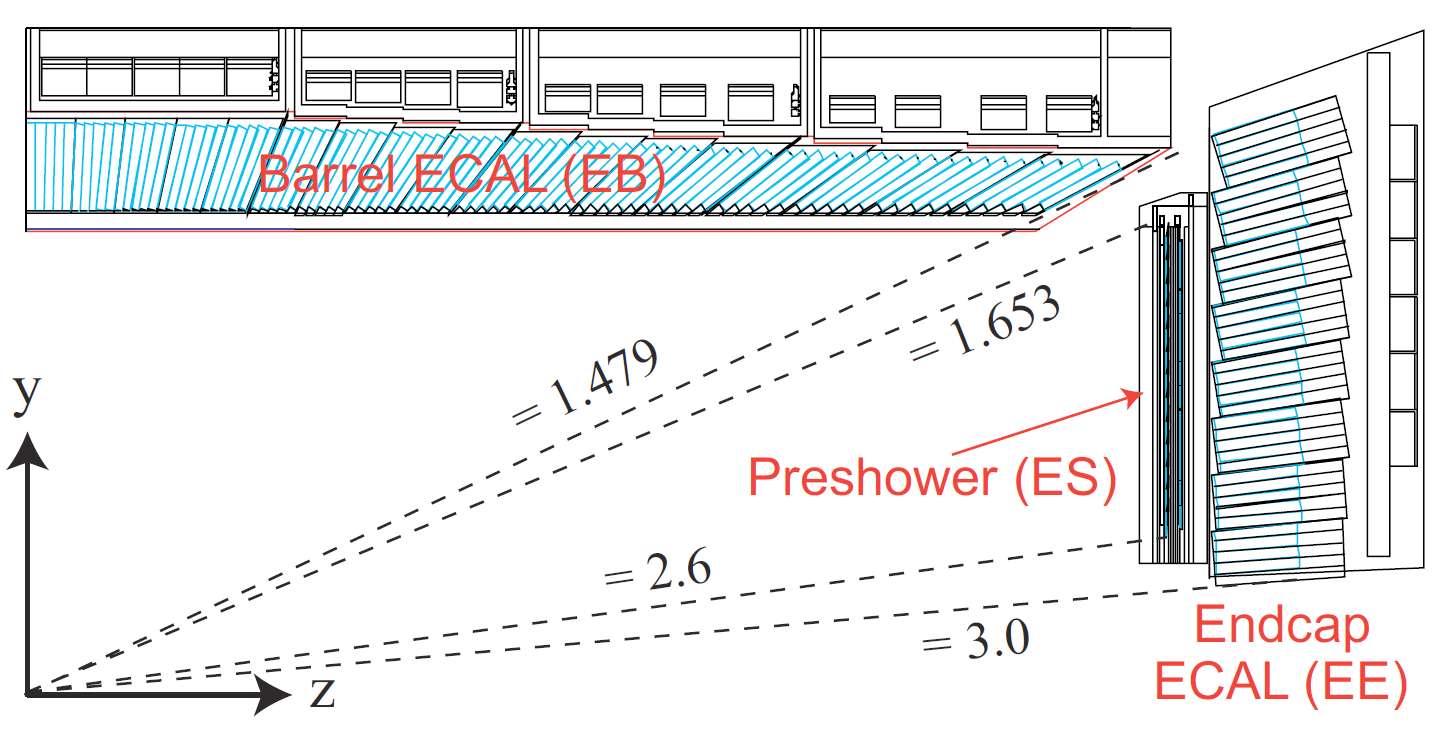
\includegraphics[width=\textwidth]{Figures/CMSECAL2}
	\caption[A geometrical quarter view of the CMS ECAL, highlighting the Barrel, Endcap and Preshower regions.]{A geometrical quarter view of the CMS ECAL, highlighting the Barrel, Endcap and Preshower regions. Figure taken from \cite{CMSTDRV1}.}
	\label{fig:CMSECAL}
\end{figure}
% http://cms-project-ecal-p5.web.cern.ch/cms-project-ECAL-P5/approved/detector.htm
A total of 75848 lead tungstate (\PbWO{}) scintillating crystals are used in the ECAL barrel and endcaps.
In the barrel section, the crystals are laid out in an $\eta-\phi$ grid extending to $\abseta<1.479$.
The inner surface of the barrel is at $r=1.29\m$, with each crystal having a front surface area of $2.2\times2.2\cmsq$ and length 23\cm{}.
In each endcap, the crystals are instead laid out in a $x-y$ grid, with the front surfaces at $z=\pm 3.14\m$, extending through $1.479 < \abseta < 3.0$. 
Each endcap crystal has a front surface area of $2.9\times2.9\cmsq$ and a length of 22\cm{}.
All the crystals are slightly off-center with respect to the primary interaction point to avoid particles being lost down the small gaps between adjacent crystals.

\PbWO{} is an ideal choice for the CMS ECAL due to its short radiation and Moli\`ere lengths at 0.89\cm{} and 2.2\cm{} respectively. 
The radiation length gives a measure of the penetration of the EM shower in the crystal and the Moli\`ere length, how confined the EM shower is, such that a cascade will mostly be contained within one crystal. 
In addition, \PbWO{} crystals are very fast, with 80\% of the blue-green scintillation light being emitted in the time it takes for another collision to occur.
The light emission from the \PbWO{} crystals is relatively small (30\photon{}/\MeV{}) and needs to be amplified using silicon avanlanche photodiodes (barrel) and vacuum phototriodes (endcaps).
\PbWO{} is also radiation resistant (10\unit{Mrad}).
% What the hell are the APD and VPT and how do they work?

The purpose of the ECAL preshower detector is to identify high energy photon depositions in the ECAL endcaps with respect to reducible, identical signatures; primarily from $\pi^{0}\rightarrow\photon{}\photon{}$ decay where $\theta_{\photon{}\photon{}}$ is small. 
To do this, the preshower consists of two layers of lead which initiate an electromagnetic shower for photons (and electrons), each closely followed by a layer of silicon strip detectors. 
The silicon strips are placed orthogonal to each other to measure shower positions precisely and are fine enough in granularity to differentiate between a single photon shower and multiple close-spaced photons.
A $\pi^{0}$ decaying in the barrel has low enough energy not to need the additional resolution provided by the preshower detector. 
The preshower degrades the resolution of the ECAL endcap due to the dense lead plates, however as the energy deposited within the lead is proportional to that deposited in the silicon, a correction can be applied mitigating the effect.
% http://www.hephy.at/project/cms/trigger/globalTrigger/trans/MEDIEN/Publications/CMSBooklet/Info_for_CMSBooklet/PreshowerFAQ_files/CMS3d.html

These attributions mean that the ECAL can be both compact enough to fit within the magnet and granular enough to perform with high energy resolution.
The resolution performance is measured by fitting a Gaussian function to reconstructed energy distributions at different test beam energies and is parameterised by Eq.\,\ref{eq:ECALRes}, where $S$ is the stochastic term (e.g. number of photoelectrons), $N$ is the noise term (e.g. electronics and digitization) and $C$ is a constant term (e.g. leakage from the back of the ECAL).
% stochastic: having a random probability distribution or pattern that may be analysed statistically but may not be predicted precisely.
% S: statistical based, photoelectrons
% N: electronics. digitization
% C: leakage, nonuniformities in crystal
Figure \ref{fig:CMSECALRes} shows the energy resolution for incident electrons at a test beam measurement. In addition, values for $S$, $N$ and $C$ are shown.
\begin{equation} \label{eq:ECALRes}
	\left(\frac{\sigma}{E}\right)^{2} = \left(\frac{S}{\sqrt{E}}\right)^{2} + \left(\frac{N}{E}\right)^{2} + C^{2}
\end{equation}
\begin{figure}[htpb]
	\centering
	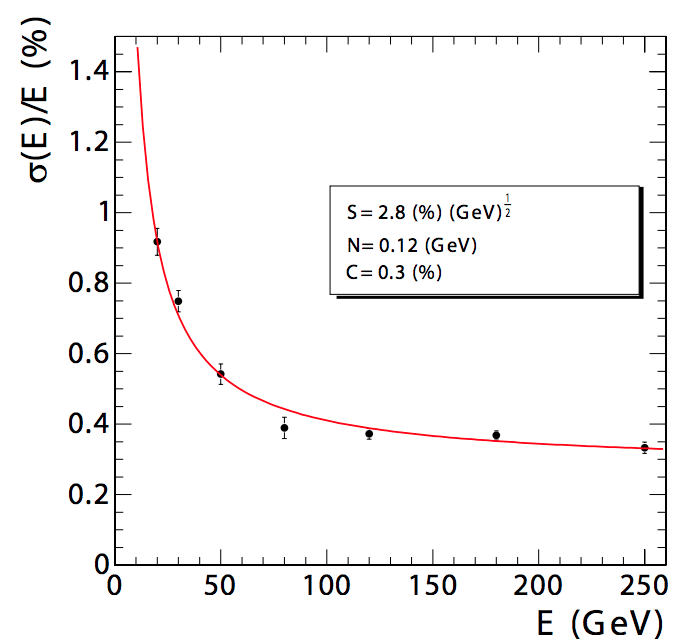
\includegraphics[width=0.7\textwidth]{Figures/CMSECALRES}
	\caption[The energy resolution of the CMS ECAL, measured from a beam test. The energy was measured in a $3\times3$ crystal lattice with the electron striking the central crystal.]{The energy resolution of the CMS ECAL, measured from a beam test. The energy was measured in a $3\times3$ crystal lattice with the electron striking the central crystal. Figure taken from \cite{CMSExperiment}.}
	\label{fig:CMSECALRes}
\end{figure}

The most recent public measurement of the ECAL resolution was taken using $Z\rightarrow e^{+}e^{-}$ data events and was $<2\%$ for $\abseta<0.8$ and  $2-5\%$ elsewhere \cite{CMSECALRESMEAS}.
% Not public measurements at 13TeV?

% 61200 in the barrel, 7324 in each endcap 
% Each crytal covers 0.0174 (1deg) in phi and eta.
% Actually 2.86 cm.
% Barrel is structured as 36 identical “supermodules,” each covering half the barrel length and corresponding to a pseudorapidity interval of 0 < |η| < 1.479. The crystals are quasi-projective (the axes are tilted at 3◦ with respect to the line from the nominal vertex position) ∆η. 
% The endcaps (EE), at a distance of 314 cm from the vertex and covering a pseudorapidity range of 1.479 < |η| < 3.0, are each structured as 2 “Dees”, consisting of semi-circular aluminium plates from which are cantilevered structural units of 5×5 crystals, known as “supercrystals.”


\subsection{Hadronic calorimeter}
\label{ssec:HCAL}

% The \MET can be inferred from all the deposits in the HCAL combined with all the deposits the ECAL.
The majority of the hadronic calorimeter (HCAL), shown in Fig. \ref{fig:CMSHCAL}, sits within the superconducting solenoid. 
It is formed of the barrel (HB), the outer barrel situated outside the solenoid (HO), and two endcaps (HE). 
The HB operates to an $\abseta<1.4$, with the HE extending the range to $\abseta<3$.
Forward hadronic detectors (HF) are situated $\pm11.2\m$ from the primary interaction point, with a pseudorapidty range of $3<\abseta<5$.
\begin{figure}[htpb]
	\centering
	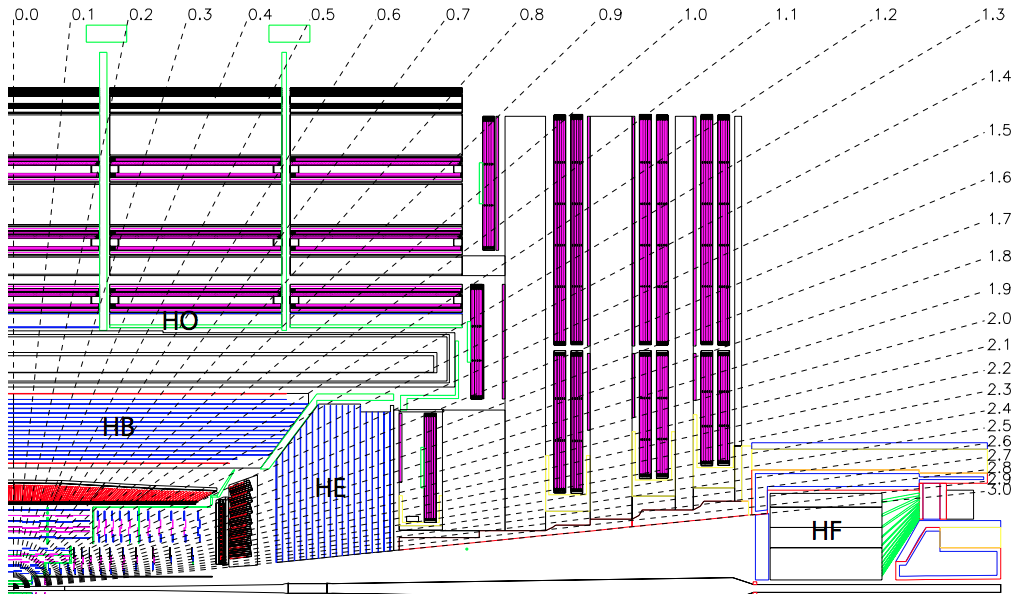
\includegraphics[width=\textwidth]{Figures/CMSHCAL}
	\caption[A geometrical quarter view of CMS HCAL, highlighting the Barrel (HB), Endcap (HE), Forward (HF) and Outer (HF) subdetectors.]{A geometrical quarter view of CMS HCAL, highlighting the Barrel (HB), Endcap (HE), Forward (HF) and Outer (HF) subdetectors. Figure taken from \cite{CMSExperiment}.}
	\label{fig:CMSHCAL}
\end{figure}

The HB, HE and HO are sampling calorimeters, composed of layers of non-magnetic, short radiation-length brass absorber and plastic scintillator tiles.
When hadrons pass through the ECAL, they leave only minimal deposits before entering the HCAL. 
When passing through the dense absorbtion layers, they interact and produce cascades of particles. 
These particle showers cause the plastic scintillator to emit blue-violet light, which is passed by very small wavelength-shifting fibres as green light to the readout where the signal is amplified using hybrid photodiodes.
At small \abseta{}, the stopping power of the HB is not enough to fully encapsulate the full hadronic cascade, so the HO is composed of scintillator tiles that are placed outside the solenoid. 
The HO improves the \MET{} resolution of the detector, by catching the tails of the hadronic cascades.
The HF, beam so close to the beam line, receives large fluxes of partciles and must be very radiation resistant.
To this end it is made of steel and quartz fibres, where the emitted Cherenkov light in the quartz fibres is passed to photomultipliers and read as signal \cite{HF}.
% Inside the magnet need as much stopping power as possible - lots of short radiation length material, thin scintillating tiles (3.7mm)

The resolution of hadronic cascades for different \abseta{} regions are shown in Fig~\ref{fig:CMSHCALRes}. 
They are given in terms of reconstructed jet energy, where a jet is a cone of particles identified from calorimeter and tracker information. 
Jet clustering will be discussed in Section TODO.
\begin{figure}[htpb]
	\centering
	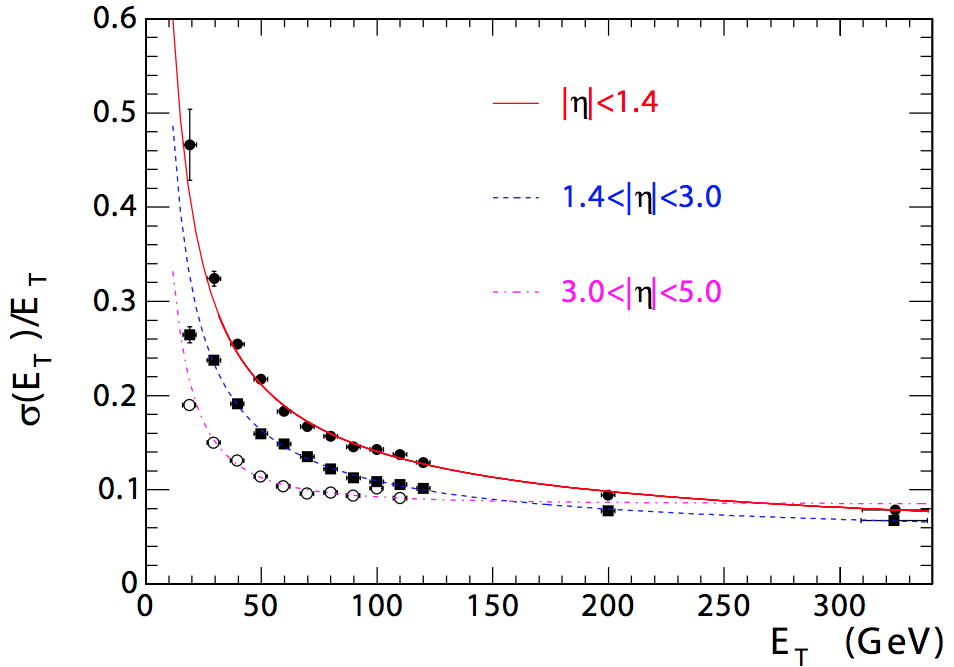
\includegraphics[width=0.7\textwidth]{Figures/CMSHCALRES}
	\caption[The transverse energy resolution of reconstructed jets in the CMS HCAL. It is split into the barrel jets ($\abseta<1.4$), endcap jets ($1.4<\abseta<3.0$) and forward jets ($3.0<\abseta<5.0$)]{The transverse energy resolution of reconstructed jets in the CMS HCAL. It is split into the barrel jets ($\abseta<1.4$), endcap jets ($1.4<\abseta<3.0$) and forward jets ($3.0<\abseta<5.0$) Figure taken from \cite{CMSExperiment}.}
	\label{fig:CMSHCALRes}
\end{figure}

\subsection{Superconducting magnet}
\label{ssec:Magnet}
% http://iopscience.iop.org/article/10.1088/1748-0221/5/03/T03021/pdf

The solenoid at the heart of CMS is the largest superconducting magnet that has ever been built at 13\m{} long and 6\m{} in diameter.
It is composed from coils of a niobium-titanium alloy wire that are cooled to an operating temperature of 4.5\Kelvin{}. 
It operates at a field strength 3.8\Tesla{}, reduced from a design operation field strength of 4\Tesla{}, in order to maximise longevity.
The magnet and steel return yokes, which are used to contain the magnetic field, are the most massive components in CMS weighing approximately 12,000 tonnes.
The high field strength allows for very precise measurements of the curvature of charged tracks leading to precise measurements of the momenta of charged particles, which is also very useful for particle identification 

\subsection{Muon detectors}
\label{ssec:MuonChambers}

The muon chambers are the outermost set of detectors at CMS, interleaved with the steel return yoke of the superconducting solenoid.
There are three types of muon chambers present at CMS; resistive plate chambers (RPC), cathode strip chambers (CSC) and drift tubes (DT).
The layout of the muon chambers is presented in Fig./,\ref{fig:CMSMuon}.
\begin{figure}[htpb]
	\centering
	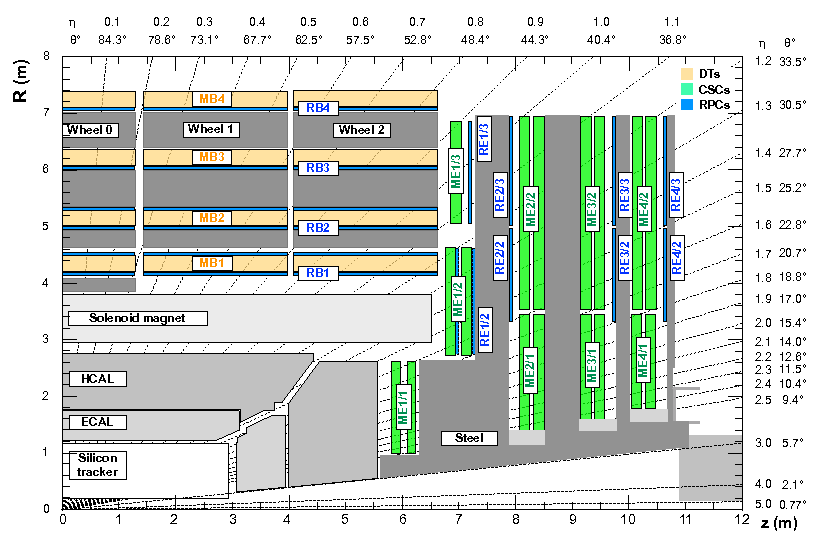
\includegraphics[width=0.9\textwidth]{Figures/CMSMUON}
	\caption[A geometrical one-quarter view of the CMS muon subsystems. In green in the barrel are the drift tubes (DT), in blue in the endcaps are the cathode strip chambers (CSC) and in red the complimentary resistive plate chambers (RPC).]{A geometrical one-quarter view of the CMS muon subsystems. In green in the barrel are the drift tubes (DT), in blue in the endcaps are the cathode strip chambers (CSC) and in red the complimentary resistive plate chambers (RPC). Figure taken from\,\cite{CMSMuon7TeV}.}
	\label{fig:CMSMuon}
\end{figure}
All three chambers are based on gas ionisation.
In the barrel, 250 DTs are used arranged in four layers for each of the five barrel wheels, out to an $\abseta<1.2$.
This is due to the conditions in the barrel, comprised of a relatively low local magnetic field strength (caused by most magnetic flux being returned through the steel yoke) and naturally low muon rates.
The DTs have a high spatial resolution, however a slow response rate of up to 380\ns{}.
% Maximum drift time of 380ns in a gas mixture of 15% CO2 85% Ar Fig 7.27
% Still very low occ (no mulithits) but large enough to be cost effective
% https://cds.cern.ch/record/1129810/files/jinst8_08_s08004.pdf
In the higher muon rate conditions of the endcap, there are 540 CSCs covering $0.9<\abseta<2.4$. 
CSCs have a quicker response time than DTs, have finer granularity and are also less affected by varying magnetic field strength found there.
% 40% Ar 50% CO2 10% CF4
Finally, 610 RPCs are found in both the barrel (six layers) and endcaps (three layers) up to $\abseta<1.6$.
The RPCs do not have very good spatial resolution, however they are very complimentary to the DTs and CSCs due to their very fast response time (much quicker than the time it takes for the next collision).
This makes the RPCs fantastic muon triggering detectors.
%  96.2% (C2H2F4), 3.5% i-C4H10 and 0.3% SF6

Figure\,\ref{fig:CMSMuonRes} shows the momentum resolution of the muon system based on tracker information only, muon chamber information only and a combination of tracker and muon chamber information.

% TODO GEMS?
\begin{figure}[htpb]
	\centering
	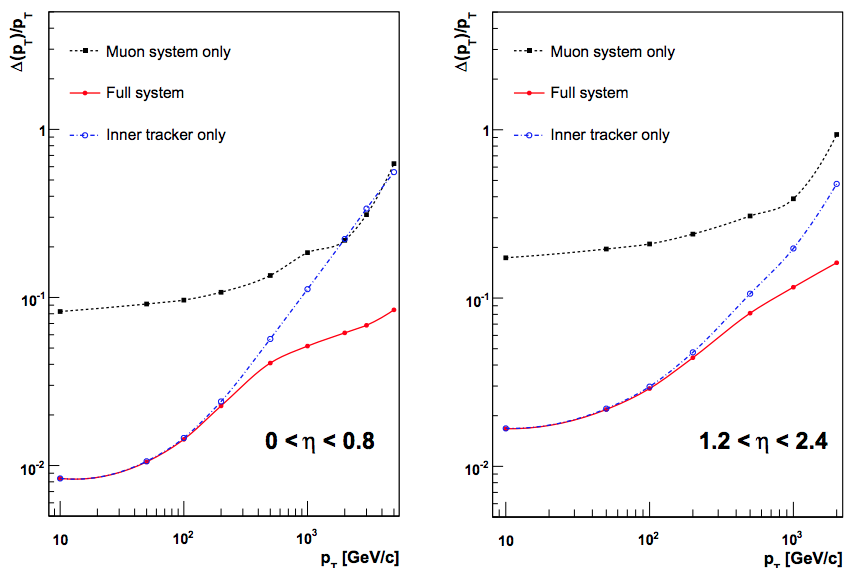
\includegraphics[width=0.85\textwidth]{Figures/CMSMUONRES}
	\caption[The muon \pt{} resolution as a function of \pt{} using the tracking only, muon subdetectors only or both.]{The muon \pt{} resolution as a function of \pt{} using the tracking only, muon subdetectors only or both. Figure taken from\,\cite{CMSExperiment}.}
	\label{fig:CMSMuonRes}
\end{figure}
% Is this figure expected or data? I think expected...

\subsection{Triggers}
\label{ssec:Trig}

The CMS detector produces events at an approximate rate of 40\MHz{}. 
If each reconstructed event has a size of $\sim 1\unit{MB}$, then data would be produced at a rate of 40\unit{TBs}$^{-1}$. 
It is unfeasible to process and store the full rate of data production, so a method of data reduction, called triggering, is used. 
Triggering decides on an event-by-event basis, whether a collision is likely to be highly-energetic and interesting, or just an elastic collision or low-energy QCD process. 
There are two types of triggering systems at CMS, the Level-1 hardware triggers (L1T) and the High-Level software triggers (HLT). 

The L1T operates at the collision rate of 40\MHz{}, with a latency of 3.2\us{} such that it is able to make a decision per event. 
It uses basic information from the detector to look for signs of interesting events, such as large calorimeter deposits or muon chamber hits.
It reduces the event rate to 100\unit{kHz}, which provides enough time for the events to be fully reconstructed before being passed to the HLT. 
The outcome of the L1T system form the \textit{seeds} for the HLT. 
The HLT, with access to the L1 seeds, full collision kinematics and composition, reduces the final physics production rate to 1\unit{kHz} and categorises the remaining events with respect to specific signatures, such as events containing a single electron, to form datasets with similar topologies.

\subsection{Computational power} % (fold)
\label{sub:computational_power}
\begin{itemize}
	\item TODO 
	\item TOTAL STORAGE, 
	\item TOTAL PROCESSING, 
	\item REQUIRE WLCG, 
	\item DESCRIPTION over 200\unit{Pb} have been produced and stored on tape at Cern 
\end{itemize}

The complete set of datasets are all stored at a Tier-0 computing facility at CERN. Most countries affliated to CMS have a large Tier-1 storage facility, storing most of the datasets, such that there are multiple redundancies for every dataset. Tier-2 and Tier-3 sites primarily only store datasets useful for locally based analysis teams, however any dataset can be accessed from any site which has it stored.
This connection of sites is collectively known as the Grid.
The distributed nature of the file system and similar environments of the host sites that goes with it, allows for any person to use free computational power anywhere that is part of the Grid, increasing the overall computational efficiency of CMS.

% subsection computational_power (end)

% Figure~\ref{CMSL1T} shows the 

% \begin{figure}[htpb]
% 	\centering
% 	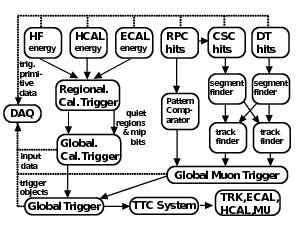
\includegraphics[width=0.7\textwidth]{Figures/CMSL1T}
% 	\caption[This needs a caption TODO Add ref in text]{This needs a caption TODO Add ref in text \cite{CMSL1T}.}
% 	\label{fig:CMSL1T}
% \end{figure}

% \subsection{UpgradesToCome}
% \label{ssec:Upgrade}
% Track Trigger?
% \subsection{DataTaken}
% \label{ssec:DataTaken}